\documentclass[a4paper,headlines=4, footlines=1]{scrartcl}
\usepackage{amsmath,amssymb,amsthm,booktabs,braket,graphicx,hyphenat,lmodern,marginnote,microtype,scrpage2,tikz,tikz-3dplot}
\usepackage[utf8]{inputenc}
\let\marginpar\marginnote{}\usepackage[ngerman]{babel}\usepackage[german=quotes]{csquotes}\usepackage[T1]{fontenc}\usepackage{hyperref}\hypersetup{colorlinks=true,linkcolor=black,citecolor=black,filecolor=black,urlcolor=black}\newcommand{\E}{\mathrm{e}}\newcommand{\I}{\mathrm{i}}\newcommand{\de}{\mathrm{d}}\newcommand{\td}[2]{\frac{\de{#1}}{\de{#2}}}\pagestyle{scrheadings} \clearscrheadings\renewcommand{\headfont}{\normalfont}
%\lehead{\pagemark}
%\cehead{}
%\rehead{\headmark}
%\lohead{\rightmark}
%\cohead{}
%\rohead{\pagemark}
\setheadsepline{0.4pt}\setfootsepline{0.4pt}
\usepackage[inner=20mm,marginparsep=5mm,marginparwidth=30mm,outer=30mm,top=30mm,bottom=30mm,footskip=10mm]{geometry}
\usepackage[format=plain,margin=3em,font=small,labelfont=bf,labelsep=endash]{caption}
\renewcommand*{\marginfont}{\footnotesize} %\renewcommand{\vec}{\mathbf}
%\usepackage{kpfonts}
\usetikzlibrary{angles,quotes}
\usepackage{extarrows}
\newcommand{\ray}[1]{\stackrel{\rightharpoonup}{#1}}
\usepackage{tabularx}
\usepackage{tkz-fct}
\usepackage{multirow}
\usepackage{enumerate}
\addto\captionsngerman{%	
	\renewcommand{\figurename}{Abb.}	
	\renewcommand{\tablename}{Tab.}	
}

\ihead{Eberhard Karls Universität Tübingen\\
	Mathematisch-Naturwissenschaftliche Fakultät\\
	Fachdidaktik II: Geometrie\\
	Prof. Dr. Hermann Hähl}
\chead{}
\ohead{\parbox[l]{2.5cm}{A. Bucher\\
		P. Gepperth\\
		S. Jung\\
		J. Stigler}}

\ifoot{Sitzung 2: Zentrische Streckungen}
\cfoot{}
\ofoot{\pagemark}


\title{Handout}

\subtitle{Strahlensätze}

\author{Pascal Gepperth}

\date{\today}

\hypersetup{
    pdftitle={Handout Fachdidaktik Mathematik Strahlensätze},
    pdfauthor={Pascal Gepperth},
	pdfstartview={FitH},
    pdfcreator={LaTeX with TikZ}
}
\begin{document}
\section*{Ähnlichkeitssätze am Kreis}
\begin{minipage}[b]{0.5\textwidth}
	\underline{\textbf{Sehnensatz am Kreis}}\\
	Schneiden sich zwei Sehnen in einem Kreis, so ist das Produkt der jeweiligen Sehnenabschnitte eine Konstante. 
	Also in der Skizze gilt:$ |A_1S|\cdot|B_2S|=|A_2S|\cdot|B_1S| $ 	
\end{minipage}
\begin{minipage}{0.5\textwidth}
	\begin{flushright}
		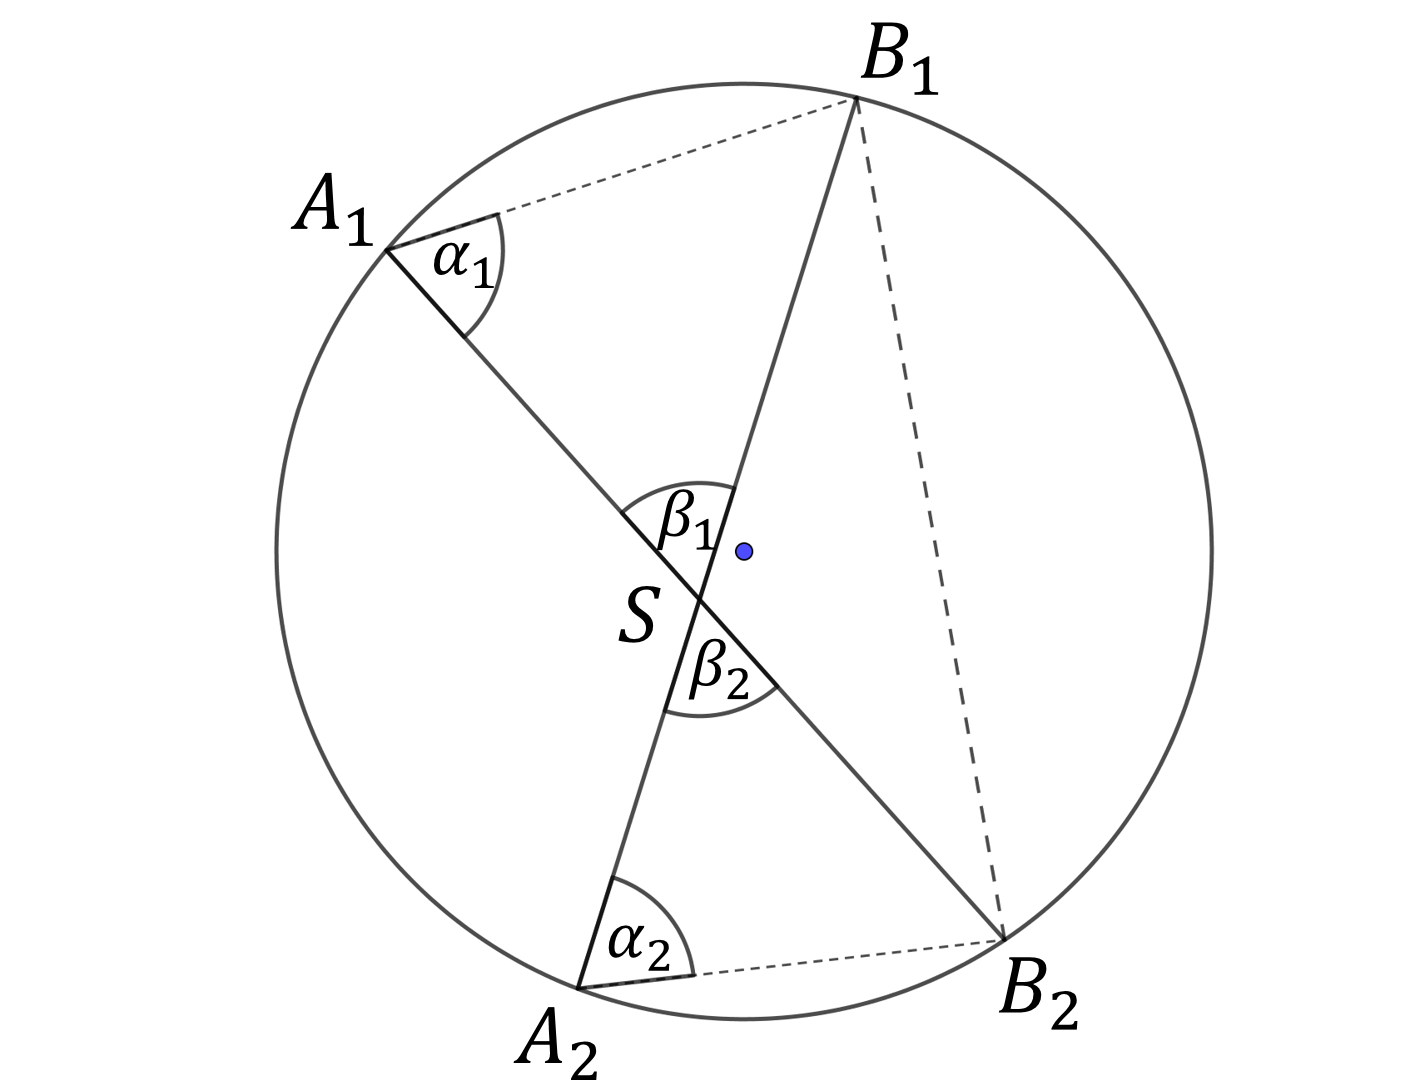
\includegraphics[scale=0.15]{Sehnensatz}
	\end{flushright}		
\end{minipage}	
\begin{minipage}[b]{0.5\textwidth}
	\underline{\textbf{Sekantensatz am Kreis}}\\ Schneiden sich zwei Sekanten außerhalb eines Kreises, so ist das Produkt der jeweiligen Sekantenabschnitte eine Konstante. 
	Also in der Skizze gilt: \\ $ |A_1S|\cdot|B_1S|=|A_2S|\cdot|B_2S| $	
\end{minipage}
\begin{minipage}{0.5\textwidth}
	\begin{flushright}
		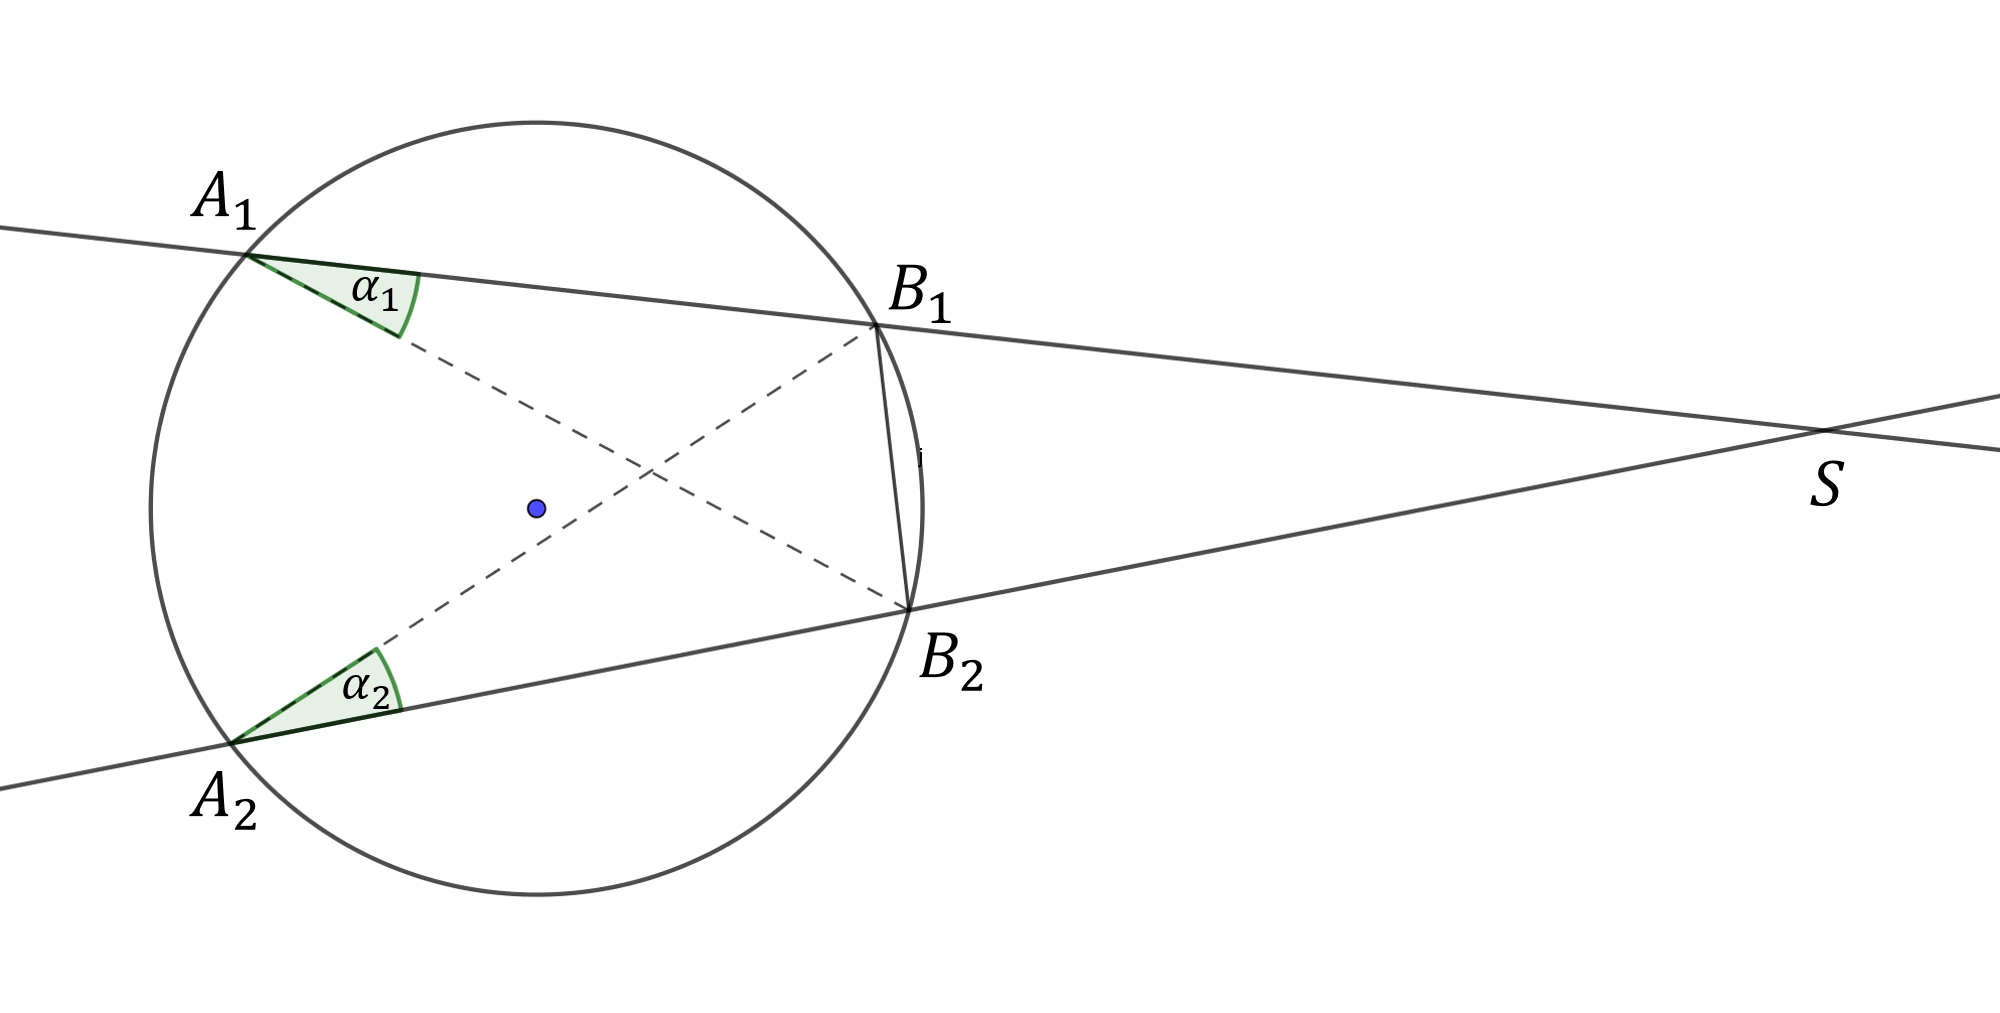
\includegraphics[scale=0.18]{Sekantensatz}
	\end{flushright}		
\end{minipage}	
\begin{minipage}[b]{0.5\textwidth}
	\underline{\textbf{Sekantentangentensatz am Kreis}}\\ Schneiden sich eine Sekante und eine tangente außerhalb eines Kreises, so ist das Produkt der Sekantenabschnitte gleich dem Quadrat des Tangentenabschnitts. 
	Also in der Skizze gilt:\\$ |A_1S|^2=|A_2S|\cdot|B_2S| $ 	
\end{minipage}
\begin{minipage}{0.5\textwidth}
	\begin{flushright}
		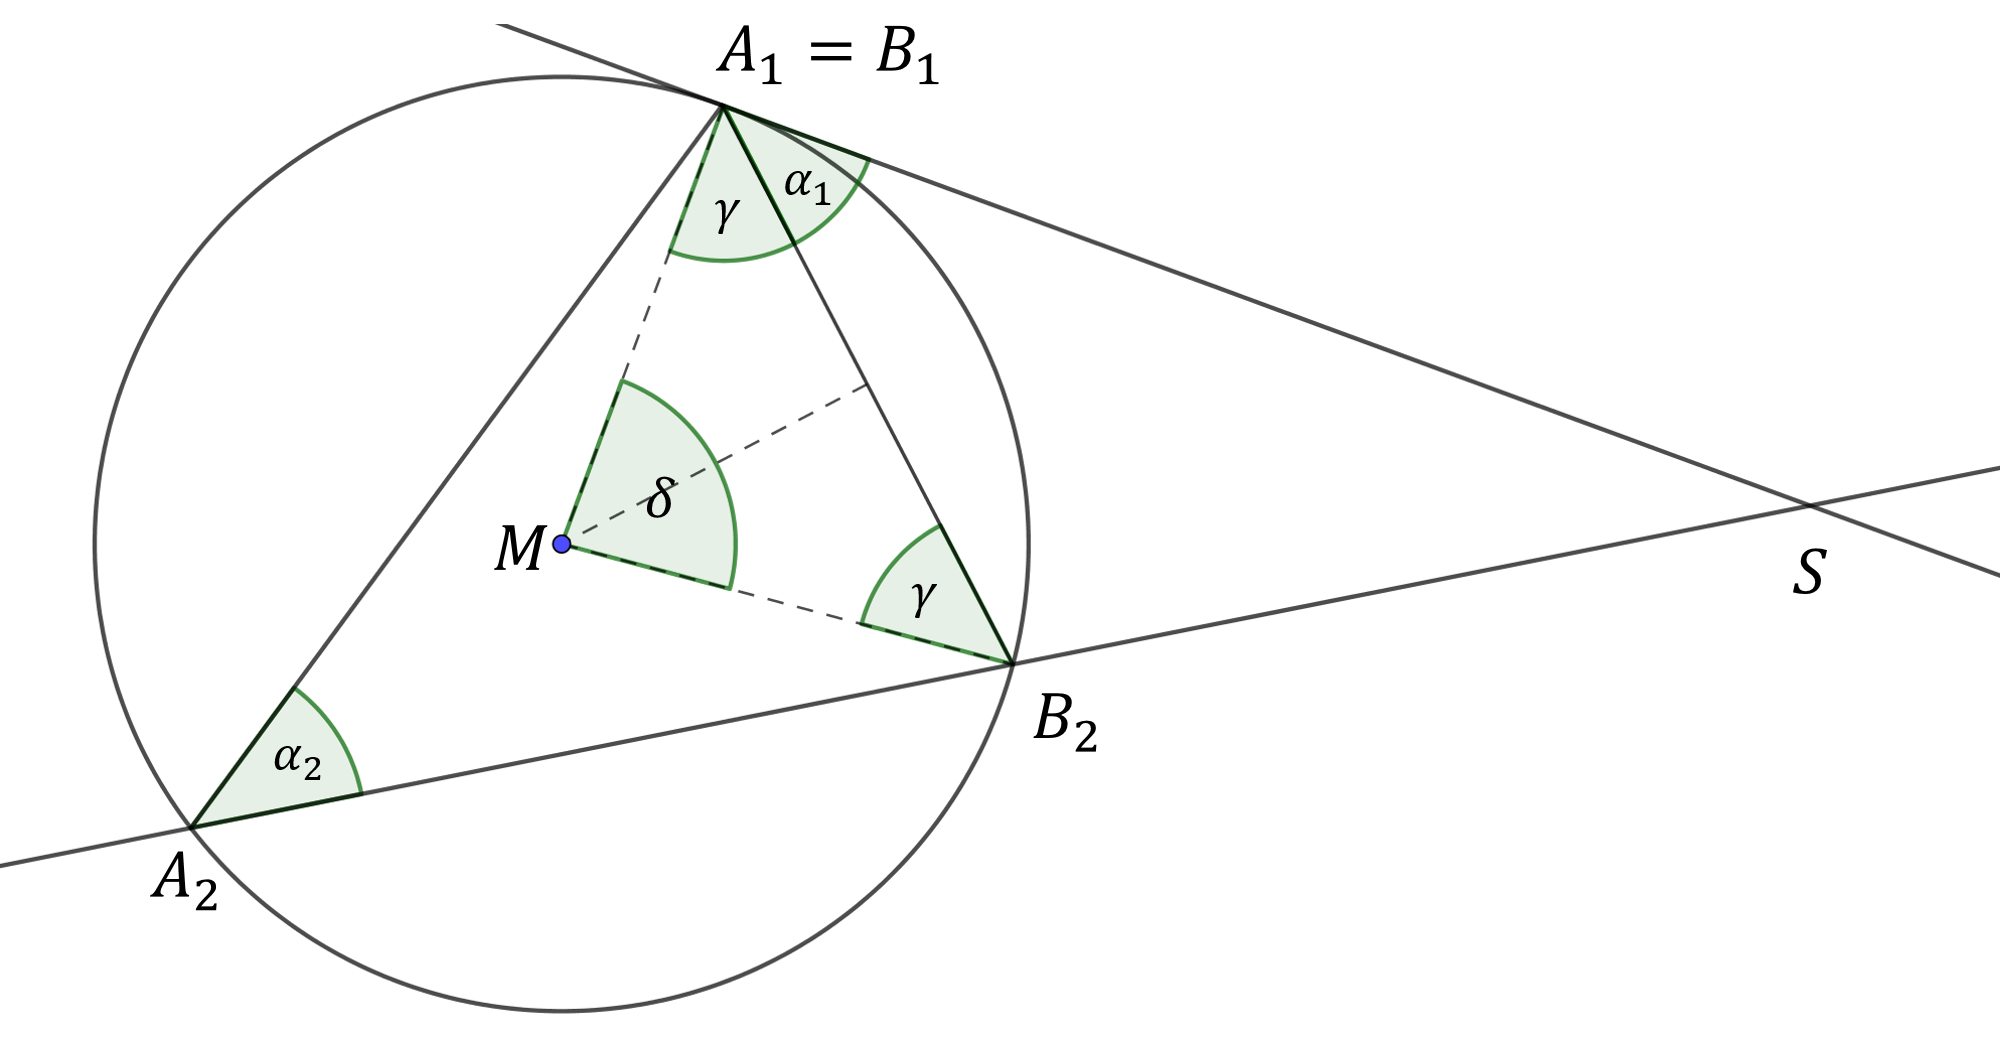
\includegraphics[scale=0.15]{Sehnentangentensatz}
	\end{flushright}		
\end{minipage}
\begin{minipage}[b]{0.5\textwidth}
	\underline{\textbf{Höhenschnittpunktsatz am Dreieck}}\\ Im Dreieck zerlegt der Höhenschnittpunkt die Höhen so, dass das Produkt der Höhenabschnitte bei allen drei Höhen konstant ist
\end{minipage}
\begin{minipage}{0.5\textwidth}
	\begin{flushright}
		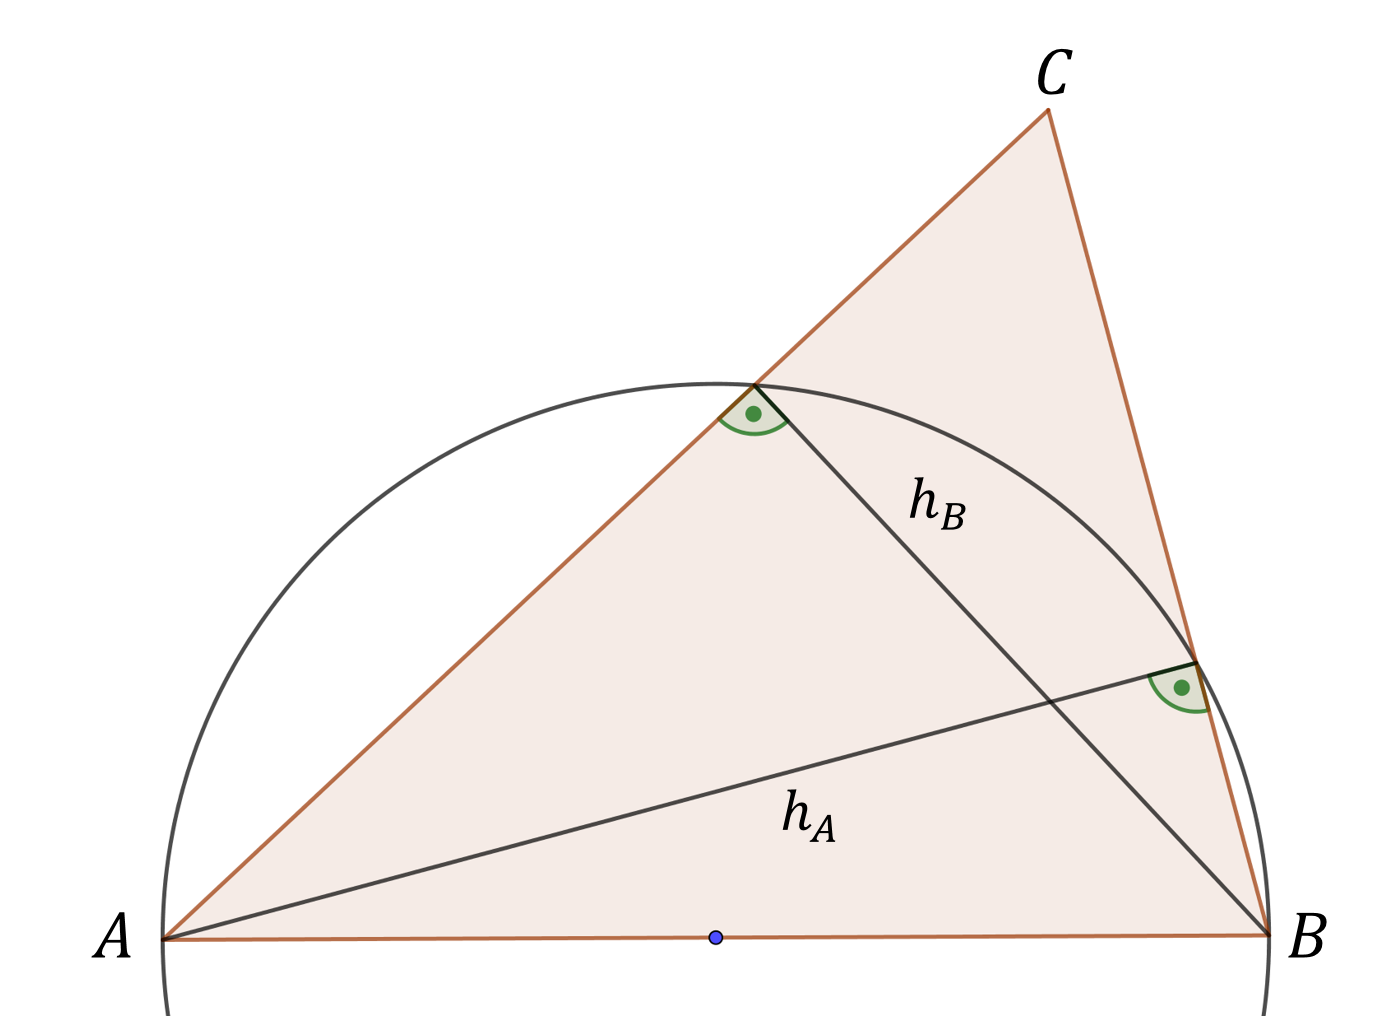
\includegraphics[scale=0.17]{Hohenabschnittsatz}
	\end{flushright}		
\end{minipage}
\end{document}
